\documentclass[a4paper]{article}
\usepackage[margin=2cm]{geometry}
\setlength\parindent{0pt}
\setlength{\parskip}{1em}

\usepackage{amsmath}
\usepackage{amssymb}
\usepackage{amsthm}
\usepackage{amsfonts}
\usepackage{bm}
\usepackage{commath}

% Column vectors
\newcount\colveccount
\newcommand*\colvec[1]{
	\global\colveccount#1
	\begin{pmatrix}
		\colvecnext
	}
	\def\colvecnext#1{
		#1
		\global\advance\colveccount-1
		\ifnum\colveccount>0
			\\
			\expandafter\colvecnext
		\else
		\end{pmatrix}
	\fi
}

% Vector norm
\newcommand{\Norm}[1]{
	\left\lVert#1\right\rVert
}

% Inner product
\newcommand{\innerp}[2]{
	\langle #1,#2 \rangle
}

\usepackage{tikz}
\usetikzlibrary{arrows, calc}
\usepackage{float}

\title{Calculations}

\begin{document}
\maketitle
\section{Collision of Two Spherical Particles Moving at Constant Velocities}
Two spherical particles with radii $R_{1}$ and $R_{2}$, have initial positions $\bm{x}^{0}_{1}$ and $\bm{x}^{0}_{2}$ and move with constant velocities $\bm{v}_{1}$ and $\bm{v}_{2}$, respectively. At what time, if at all, will they collide?

\begin{figure}[H]
	\centering
	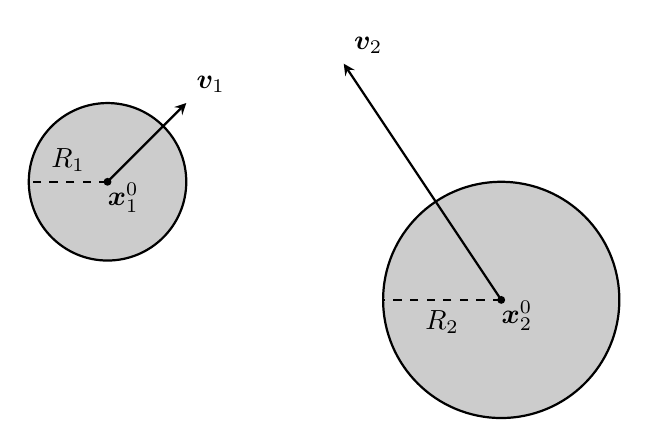
\begin{tikzpicture}
		\coordinate (x1) at (0,0);
		\draw[thick, fill=black!20] (x1) circle (1);
		\fill[black] (x1) circle (0.05);
		\draw[->, >=stealth, thick] (x1) -- ++(1,1) node [above right] {$\bm{v}_{1}$};
		\draw[dashed, thick] (x1) -- ++(-1,0) node [midway, above] {$R_{1}$};
		\node at (0.2,-0.2) {$\bm{x}^{0}_{1}$};
		
		\coordinate (x2) at (5,-1.5);
		\draw[thick, fill=black!20] (x2) circle (1.5);
		\fill[black] (x2) circle (0.05);
		\draw[->, >=stealth, thick] (x2) -- ++(-2,3) node [above right] {$\bm{v}_{2}$};
		\draw[dashed, thick] (x2) -- ++(-1.5,0) node [midway, below] {$R_{2}$};
		\node at ($(x2)+(0.2,-0.2)$) {$\bm{x}^{0}_{2}$};
	\end{tikzpicture}
\end{figure}

The position of particle 1 as a function of time is
\begin{equation}
	\bm{x}_{1}(t) = \bm{x}^{0}_{1} + \bm{v}_{1}t,
	\label{eq:p1_pos}
\end{equation}
The position of particle 2 as a function of time is identical, i.e.
\begin{equation}
	\bm{x}_{2}(t) = \bm{x}^{0}_{2} + \bm{v}_{2}t.
	\label{eq:p2_pos}
\end{equation}
Therefore, the distance $\bm{r}(t)$ between the particles is
\begin{equation}
	\bm{r}(t) = \bm{x}_{1}(t) - \bm{x}_{2}(t) = \bm{x}^{0}_{1} + \bm{v}_{1}t - \bm{x}^{0}_{2} - \bm{v}_{2}t,
	\label{eq:distance_vec}
\end{equation}
or in explicit vector form
	\begin{align}
	\bm{r}(t) &= \colvec{3}{x^{0}_{1}+v^{x}_{1}t - x^{0}_{2}+v^{x}_{2}t}{y^{0}_{1}+v^{y}_{1}t - y^{0}_{2}+v^{y}_{2}t}{z^{0}_{1}+v^{z}_{1}t - z^{0}_{2}+v^{z}_{2}t}\nonumber\\
	&= \colvec{3}{\left(x^{0}_{1}-x^{0}_{2}\right)-\left(v^{x}_{1}-v^{x}_{2}\right)t}{\left(y^{0}_{1}-y^{0}_{2}\right)-\left(v^{y}_{1}-v^{y}_{2}\right)t}{\left(z^{0}_{1}-z^{0}_{2}\right)-\left(v^{z}_{1}-v^{z}_{2}\right)t}\nonumber\\
	&= \colvec{3}{\Delta x_{0}-\Delta v^{x}t}{\Delta y_{0}-\Delta v^{y}t}{\Delta z_{0}-\Delta v^{z}t}.
		\label{eq:distance_explicit}
	\end{align}

	The square of the norm of $\bm{r}(t)$ is thus
	\begin{align}
		\Norm{r}^{2} &= \left( \Delta x_{0}-\Delta v^{x}t \right)^{2} + \left( \Delta x_{0}-\Delta v^{x}t \right)^{2} + \left( \Delta x_{0}-\Delta v^{x}t \right)^{2}\nonumber\\
		&= \left(\Delta x_{0}\right)^{2} - 2\Delta x_{0}\Delta v^{x}t + \left(\Delta v^{x}\right)^{2}t^{2} + \cdots\nonumber\\
		&= \left(\Delta x_{0}\right)^{2} + \left( \Delta y_{0} \right)^{2} + \left( \Delta z_{0} \right)^{2} - 2\left( \Delta x_{0}\Delta v^{x} + \Delta y_{0}\Delta v^{y} + \Delta z_{0}\Delta v^{z} \right)t + \left(\left( \Delta v^{x} \right)^{2} + \left( \Delta v^{y} \right)^{2} + \left( \Delta v^{z} \right)^{2}\right)t^{2}\nonumber\\
		&= \Norm{\Delta \bm{x}_{0}}^{2} - 2\innerp{\Delta\bm{x}_{0}}{\Delta\bm{v}}t + \Norm{\Delta \bm{v}}^{2}t^{2}.
		\label{eq:norm_square_dist}
	\end{align}

	The times $t_{1,2}$ for which the particles collide can be calculated by solving equation \ref{eq:norm_square_dist} for the case
	\begin{equation}
		\Norm{r}^{2} = \left(R_{1}+R_{2}\right)^{2} = R^{2},
		\label{eq:collision}
	\end{equation}
	i.e. when the distance between the particles is the sum of their radii.

	Using the quadratic formula,
	\begin{align}
		t_{1,2} &= \frac{2\innerp{\Delta\bm{x}_{0}}{\Delta\bm{v}}\pm\sqrt{4\innerp{\Delta\bm{x}_{0}}{\Delta\bm{v}}^{2} - 4\Norm{\Delta\bm{v}}^{2}\left( \Norm{\Delta\bm{x}_{0}}^{2}-R^{2} \right)}}{2\Norm{\Delta\bm{v}}^{2}}\nonumber\\
		&= \frac{\innerp{\Delta\bm{x}_{0}}{\Delta\bm{v}}\pm\sqrt{\innerp{\Delta\bm{x}_{0}}{\Delta\bm{v}}^{2} - \Norm{\Delta\bm{v}}^{2}\left( \Norm{\Delta\bm{x}_{0}}^{2}-R^{2} \right)}}{\Norm{\Delta\bm{v}}^{2}}.
		\label{eq:quad_formula}
	\end{align}

	The condition for which a collision will happen is therefore
	\begin{equation}
		\innerp{\Delta\bm{x}_{0}}{\Delta\bm{v}}^{2} \geq \Norm{\Delta\bm{v}}^{2}\left( \Norm{\Delta\bm{x}_{0}}^{2}-R^{2} \right).
		\label{eq:if_collision}
	\end{equation}
\end{document}
